\chapter{Jantung dan Daur Jantung}\label{ch:b2:heart}

Keluarkan \omterm{def:b2:heart:anatomy}{jantung} seekor katak lalu jatuhkan ia ke dalam larutan
garam, maka ia terus berdenyut selama berjam-jam --- tanpa saraf,
tanpa otak, tanpa \omterm{def:b2:blood-circulation:blood}{darah}, hanya sebuah otot yang berkerut dengan
sendirinya kira-kira sekali tiap detik karena sepetak kecil selnya
tidak sanggup diam. \omterm{def:b2:heart:anatomy}{Jantung} manusia mengerjakan hal ini kira-kira tiga
miliar kali dalam satu hidup, memindahkan sekitar dua ratus juta liter,
tanpa pernah dimatikan. Bab ini membahas pompa itu: ruang dan katupnya,
daur pengisian dan pengosongannya beserta tekanan yang
menggerakkannya, sistem kelistrikan yang mengatur waktunya dan jejak
yang ia tinggalkan pada kulitnya, hukum yang membolehkannya menyerasikan
keluarannya dengan alirannya yang masuk denyut demi denyut, serta saraf
dan hormon yang menyetel langkah dan gayanya.

\section{Pompanya}

\begin{definition}[Ruang dan katup]\label{def:b2:heart:anatomy}
\index{jantung}\index{serambi}\index{bilik}\index{katup jantung}
Jantung adalah dua pompa yang bersebelahan, masing-masing sebuah
\emph{serambi} yang menerima \omterm{def:b2:blood-circulation:blood}{darah} dari \omterm{def:b2:blood-circulation:vessels}{vena} dan sebuah \emph{bilik}
yang menyemburkannya ke dalam sebuah \omterm{def:b2:blood-circulation:vessels}{arteri}. Jantung kanan mengambil
\omterm{def:b2:blood-circulation:blood}{darah} dari \omterm{def:b2:blood-circulation:vessels}{vena} cava lalu mengirimkannya ke paru-paru lewat \omterm{def:b2:blood-circulation:vessels}{arteri}
paru; jantung kiri mengambilnya kembali dari \omterm{def:b2:blood-circulation:vessels}{vena} paru lalu
mengirimkannya berkeliling tubuh lewat aorta. Empat katup membuat
alirannya searah: \emph{katup serambi-bilik} (trikuspid di kanan,
mitral di kiri), yaitu daun katup yang ditambatkan tali kepada otot
papila sehingga ia tidak dapat tertiup balik ke dalam serambinya; dan
\emph{katup semilunar} (paru dan aorta), yaitu tiga kantung yang terisi
lalu menutup rapat ketika tekanan \omterm{def:b2:blood-circulation:vessels}{arterinya} melampaui tekanan biliknya.
Katupnya bersifat pasif: ia membuka dan menutup hanya karena beda
tekanan. Dinding biliknya adalah \emph{miokardium}, yaitu otot lurik
dari sel bercabang yang tersambung ujung dengan ujung oleh \emph{cakram
selitan} yang penuh sambungan renggang, sehingga seluruh biliknya
secara kelistrikan merupakan satu sel dan berkerut sebagai satu
kesatuan; dinding bilik kirinya tiga kali lebih tebal daripada dinding
bilik kanannya karena ia memompa melawan lima kali tekanannya. Otot
jantungnya diberi makan oleh \emph{\omterm{def:b2:blood-circulation:vessels}{arteri} koronernya} sendiri, yang
terisi pada diastolnya, dan ia berjalan hampir sepenuhnya pada
metabolisme aerob --- ia tidak dapat berutang.
\end{definition}

\begin{omfigure}
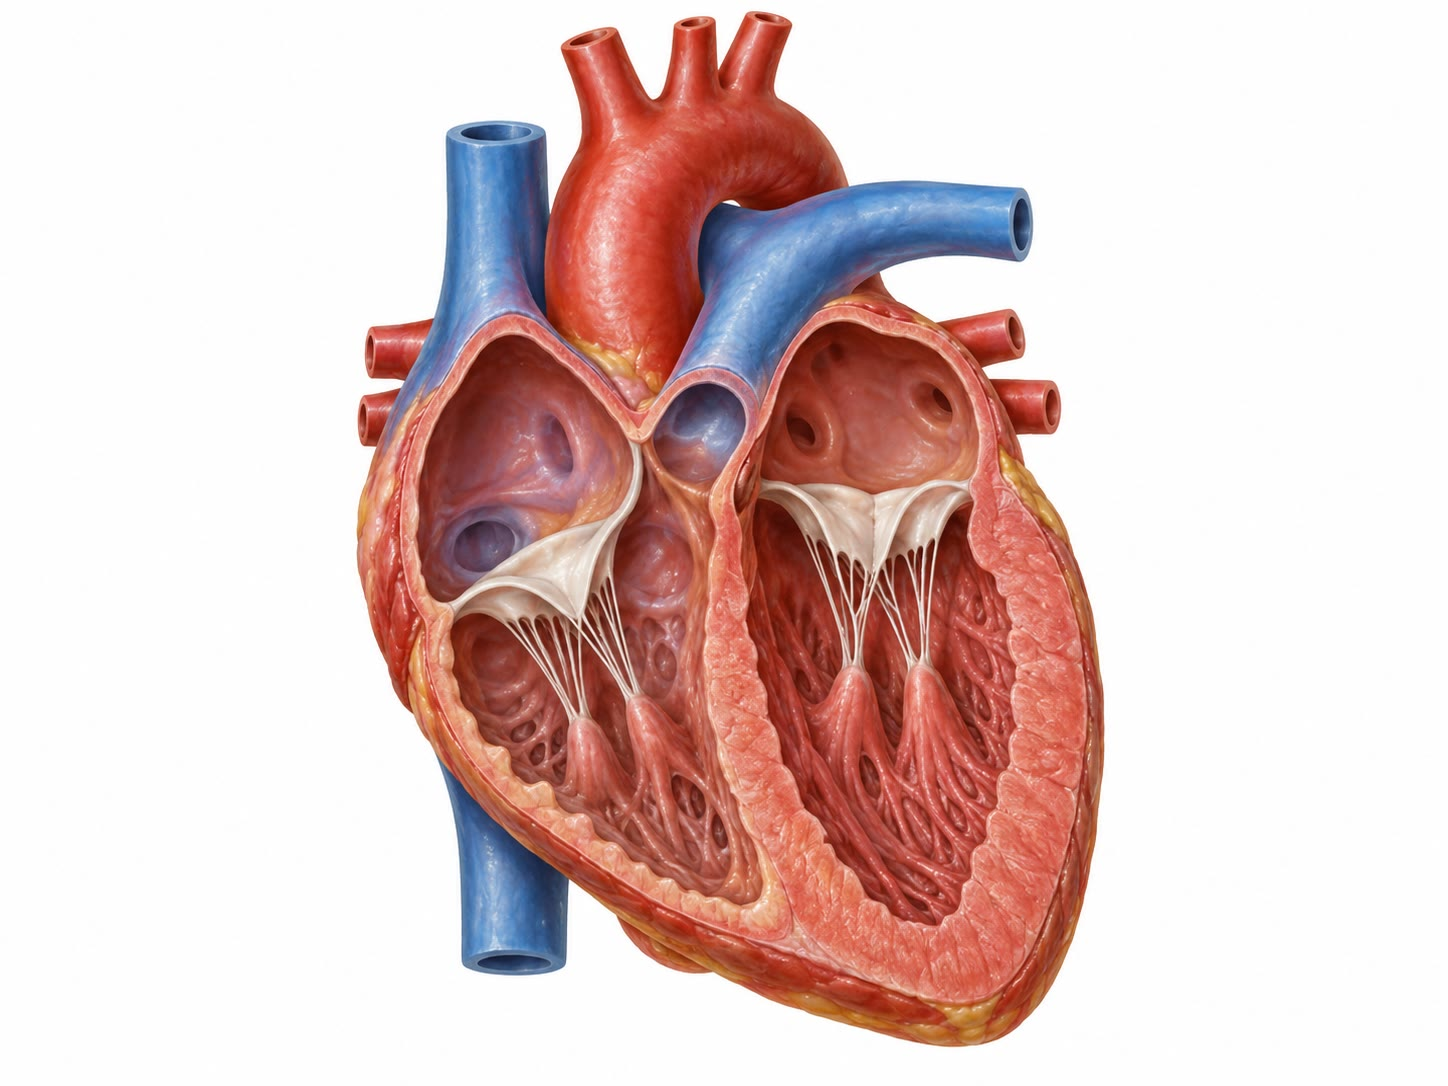
\includegraphics[width=0.55\linewidth]{images/book4/ai/b4-17-heart-cutaway.jpg}

{\small \omterm{def:b2:heart:anatomy}{Jantung} pada irisan depan: dua \omterm{def:b2:heart:anatomy}{serambi} di atas, dua \omterm{def:b2:heart:anatomy}{bilik} di
bawah, \omterm{def:b2:heart:anatomy}{bilik} kiri yang tebal, katup \omterm{def:b2:heart:anatomy}{serambi-bilik} beserta talinya, dan
kedua \omterm{def:b2:blood-circulation:vessels}{arteri} besar yang meninggalkan puncaknya.}
\end{omfigure}

\begin{proposition}[Daur jantung]\label{prop:b2:heart:cycle}
\index{daur jantung}\index{sistol}\index{diastol}\index{volume sekuncup}\index{fraksi semburan}
Satu denyut ketika beristirahat berlangsung kira-kira \qty{0.8}{s}.
\emph{Diastol} (\qty{0.5}{s}): \omterm{def:b2:heart:anatomy}{biliknya} mengendur, tekanannya turun di
bawah tekanan \omterm{def:b2:heart:anatomy}{serambinya}, katup \omterm{def:b2:heart:anatomy}{serambi-biliknya} membuka dan \omterm{def:b2:blood-circulation:blood}{darahnya}
mengalir masuk, kebanyakan secara pasif, lalu dengan sebuah dorongan
terakhir dari kerutan \omterm{def:b2:heart:anatomy}{serambinya}; \omterm{def:b2:heart:anatomy}{biliknya} mengakhiri diastolnya sambil
menahan kira-kira \qty{120}{mL} (\emph{volume akhir diastol}).
\emph{Sistol} (\qty{0.3}{s}): \omterm{def:b2:heart:anatomy}{biliknya} berkerut; begitu tekanannya
melampaui tekanan \omterm{def:b2:heart:anatomy}{serambinya}, katup \omterm{def:b2:heart:anatomy}{serambi-biliknya} menutup (bunyi
\omterm{def:b2:heart:anatomy}{jantung} pertama, ``lub''), dan selama beberapa perseratus detik
\omterm{def:b2:heart:anatomy}{biliknya} memeras sebuah ruang yang tertutup --- \emph{kerutan
isovolumetrik} --- sampai tekanannya melewati tekanan \omterm{def:b2:blood-circulation:vessels}{arterinya}
(\qty{80}{mmHg} di kiri), ketika katup semilunarnya membuka dan
\omterm{def:b2:blood-circulation:blood}{darahnya} disemburkan. \omterm{def:b2:heart:anatomy}{Bilik} kirinya mencapai \qty{120}{mmHg} dan
mengusir kira-kira \qty{70}{mL} (yaitu \emph{\omterm{prop:b2:heart:cycle}{volume sekuncupnya}},
dengan \emph{\omterm{prop:b2:heart:cycle}{fraksi semburan}} \qty{60}{\%}); ketika ia mengendur,
tekanannya turun di bawah tekanan aortanya, katup aortanya menutup
dengan bunyi ``dub'' (bunyi kedua), dan pengenduran isovolumetrik
membawa tekanannya turun sampai aras \omterm{def:b2:heart:anatomy}{serambinya}, ketika pengisiannya
dimulai lagi. \omterm{def:b2:heart:anatomy}{Jantung} kanannya mengerjakan hal yang sama pada
seperlima tekanannya, menyemburkan volume yang sama.
\end{proposition}

\begin{omfigure}
\begin{tikzpicture}
\begin{axis}[
  width=0.9\linewidth, height=7.2cm,
  axis x line=bottom, axis y line=left,
  xmin=0, xmax=0.8, ymin=0, ymax=130,
  xlabel={waktu dalam daurnya (s)}, ylabel={tekanan (\unit{mmHg})},
  xlabel style={font=\small, at={(axis description cs:0.5,-0.1)}, anchor=north},
  ylabel style={font=\small},
  tick label style={font=\small}, xtick={0,0.1,0.3,0.8}, ytick={0,40,80,120},
  legend style={font=\scriptsize, at={(0.6,0.45)}, anchor=west, draw=none},
  clip=false,
]
% aortic pressure
\addplot[very thick, omThm] coordinates {(0,82) (0.05,80) (0.1,80) (0.12,95) (0.16,115) (0.2,120) (0.25,112) (0.3,100) (0.32,104) (0.34,100) (0.45,94) (0.6,88) (0.8,82)};
\addlegendentry{aorta}
% left ventricular pressure
\addplot[very thick, omDef] coordinates {(0,5) (0.04,8) (0.05,10) (0.08,60) (0.1,80) (0.12,95) (0.16,115) (0.2,120) (0.25,112) (0.3,100) (0.32,60) (0.35,20) (0.38,5) (0.5,3) (0.7,5) (0.75,8) (0.8,5)};
\addlegendentry{bilik kiri}
% atrial pressure
\addplot[thick, omProp] coordinates {(0,6) (0.03,9) (0.06,6) (0.1,8) (0.15,6) (0.3,7) (0.36,10) (0.4,5) (0.6,6) (0.75,9) (0.8,6)};
\addlegendentry{serambi kiri}
\draw[dashed, gray] (axis cs:0.05,0) -- (axis cs:0.05,128); \node[font=\scriptsize, anchor=south, align=center] at (axis cs:0.05,128) {mitral\\menutup};
\draw[dashed, gray] (axis cs:0.1,0) -- (axis cs:0.1,128); \node[font=\scriptsize, anchor=south, align=center] at (axis cs:0.13,128) {aorta\\membuka};
\draw[dashed, gray] (axis cs:0.31,0) -- (axis cs:0.31,128); \node[font=\scriptsize, anchor=south, align=center] at (axis cs:0.31,128) {aorta\\menutup};
\draw[dashed, gray] (axis cs:0.38,0) -- (axis cs:0.38,128); \node[font=\scriptsize, anchor=south, align=center] at (axis cs:0.4,128) {mitral\\membuka};
\node[font=\scriptsize] at (axis cs:0.2,45) {sistol};
\node[font=\scriptsize] at (axis cs:0.55,25) {diastol};
\end{axis}
\end{tikzpicture}

{\small Tekanan di dalam \omterm{def:b2:heart:anatomy}{jantung} kiri sepanjang satu denyut. \omterm{def:b2:heart:anatomy}{Biliknya}
memeras sebuah ruang yang tertutup sampai ia melampaui tekanan
aortanya, menyembur selama ia berada di atasnya, mengendur sampai ia
turun di bawah tekanan \omterm{def:b2:heart:anatomy}{serambinya}, lalu terisi.}
\end{omfigure}

\begin{theorem}[Kerja jantungnya]\label{thm:b2:heart:work}
\index{kerja jantung}\index{gelung tekanan--volume}
Digambarkan sebagai tekanan terhadap volume, satu denyut \omterm{def:b2:heart:anatomy}{bilik} kirinya
menjejakkan sebuah gelung --- pengisian sepanjang dasarnya, kerutan
isovolumetrik naik di sisi kanannya, semburan sepanjang atasnya dari
\qty{120}{mL} menjadi \qty{50}{mL}, pengenduran isovolumetrik turun di
sisi kirinya --- dan luas gelungnya adalah kerja mekanis denyutnya:
\[
W = \oint P\,\mathrm{d}V \approx \bar P_{\text{semburan}}\times \text{volume sekuncup} \approx \qty{100}{mmHg}\times\qty{70}{mL} = \qty{0.93}{J}.
\]
Pada 72 denyut tiap menit \omterm{def:b2:heart:anatomy}{bilik} kirinya mengerjakan kira-kira
\qty{1.1}{W}, \omterm{def:b2:heart:anatomy}{bilik} kanannya \qty{0.2}{W}; metabolisme \omterm{def:b2:heart:anatomy}{jantungnya}
sekitar \qty{8}{W}, sehingga daya guna mekanisnya mendekati
\qty{15}{\%}, sisanya berupa panas dan ongkos tegangannya. Menaikkan
tekanan yang dilawan \omterm{def:b2:heart:anatomy}{jantungnya} ketika memompa (hipertensi, katup
aorta yang menyempit) menaikkan kerja tiap denyutnya secara sebanding,
dan ototnya menebal sebagai tanggapan sebagaimana otot mana pun ---
sampai pasokan koronernya tidak lagi sanggup mengimbangi bongkahnya.
\end{theorem}
\begin{proof}
Kerja adalah gaya kali jarak, dan bagi sebuah tekanan yang bekerja pada
dinding yang bergerak, tekanan kali volume yang tersapu: $\mathrm{d}W = P\,\mathrm{d}V$.
Sepanjang sebuah gelung tertutup kerja bersihnya adalah luas yang
dilingkupinya (pengisian pada tekanan rendah berongkos sedikit;
semburan pada tekanan tinggi mengembalikan jauh lebih banyak).
$\qty{100}{mmHg} = \qty{1.33e4}{Pa}$ dan $\qty{70}{mL} =
\qty{7e-5}{m^3}$: $1.33\times 10^{4}\times 7\times 10^{-5} =
\qty{0.93}{J}$; dikali $1.2$ denyut tiap detik, \qty{1.1}{W}.
\end{proof}

\begin{omfigure}
\begin{tikzpicture}
\begin{axis}[
  width=0.62\linewidth, height=6cm,
  axis x line=bottom, axis y line=left,
  xmin=0, xmax=150, ymin=0, ymax=140,
  xlabel={volume bilik kiri (\unit{mL})}, ylabel={tekanan (\unit{mmHg})},
  xlabel style={font=\small, at={(axis description cs:0.5,-0.12)}, anchor=north},
  ylabel style={font=\small},
  tick label style={font=\small}, xtick={0,50,120}, ytick={0,80,120},
  clip=false,
]
\fill[omDef!12] (axis cs:50,5) -- (axis cs:120,8) -- (axis cs:120,80) -- (axis cs:110,115) -- (axis cs:80,122) -- (axis cs:50,100) -- cycle;
\draw[very thick, omDef, ->] (axis cs:50,5) -- (axis cs:120,8);
\draw[very thick, omDef, ->] (axis cs:120,8) -- (axis cs:120,80);
\draw[very thick, omDef, ->] (axis cs:120,80) .. controls (axis cs:110,118) and (axis cs:80,125) .. (axis cs:50,100);
\draw[very thick, omDef, ->] (axis cs:50,100) -- (axis cs:50,5);
\node[font=\scriptsize, anchor=south] at (axis cs:85,11) {pengisian};
\node[font=\scriptsize, anchor=west] at (axis cs:122,44) {kerutan isovolumetrik};
\node[font=\scriptsize, anchor=south] at (axis cs:85,124) {semburan};
\node[font=\scriptsize, anchor=east] at (axis cs:48,52) {pengenduran};
\node[font=\scriptsize] at (axis cs:85,60) {luas $=$ kerja, \qty{0.9}{J}};
\end{axis}
\end{tikzpicture}

{\small \omterm{thm:b2:heart:work}{Gelung tekanan--volume} \omterm{def:b2:heart:anatomy}{bilik} kirinya. Luas yang dilingkupinya
adalah kerja satu denyut; tekanan \omterm{def:b2:blood-circulation:vessels}{arteri} yang lebih tinggi menaikkan
bagian atas gelungnya beserta kerjanya.}
\end{omfigure}

\section{Jam jantungnya sendiri}

\begin{proposition}[Keotomatisan dan penghantaran]\label{prop:b2:heart:conduction}
\index{nodus sinoatrium}\index{pacu jantung}\index{nodus atrioventrikel}\index{serabut Purkinje}
Denyutnya bermula di \emph{\omterm{prop:b2:heart:conduction}{nodus sinoatrium}}, yaitu sepetak sel otot
khusus di dalam dinding \omterm{def:b2:heart:anatomy}{serambi} kanan yang potensial membrannya tidak
pernah beristirahat: setelah tiap potensial aksinya ia menghanyut
perlahan ke atas (sebuah \emph{potensial pacu}, yang digerakkan arus
natrium yang menyala pada potensial negatif dan oleh kanal kalsium)
sampai ia mencapai ambangnya lalu memicu lagi, kira-kira seratus kali
tiap menit jika dibiarkan sendiri. Impulsnya menyebar lewat otot
\omterm{def:b2:heart:anatomy}{serambinya}, sel demi sel lewat sambungan renggangnya, dan \omterm{def:b2:heart:anatomy}{serambinya}
berkerut; ia mencapai \emph{\omterm{prop:b2:heart:conduction}{nodus atrioventrikel}}, yaitu satu-satunya
jembatan kelistrikan antara \omterm{def:b2:heart:anatomy}{serambi} dan \omterm{def:b2:heart:anatomy}{bilik}, yang menghantar dengan
lambat dan menundanya sepersepuluh detik --- waktu bagi \omterm{def:b2:heart:anatomy}{serambinya}
untuk merampungkan pengisian \omterm{def:b2:heart:anatomy}{biliknya}; lalu ia meluncur turun lewat
\emph{berkas His} dan \emph{\omterm{prop:b2:heart:conduction}{serabut Purkinje}}, yaitu sel penghantar
cepat yang mengantarkannya ke seluruh otot \omterm{def:b2:heart:anatomy}{biliknya} dalam
\qty{30}{ms}, sehingga \omterm{def:b2:heart:anatomy}{biliknya} berkerut dari puncaknya ke atas,
sebagai satu kesatuan, lalu mendorong \omterm{def:b2:blood-circulation:blood}{darahnya} menuju katup
keluarannya. Tiap bagian sistem ini dapat memacu sendiri, masing-masing
lebih lambat daripada yang sebelumnya (nodusnya pada 100, \omterm{prop:b2:heart:conduction}{nodus
atrioventrikelnya} pada 50, \omterm{prop:b2:heart:conduction}{serabut Purkinjenya} pada 30), sehingga jika
nodusnya gagal sebuah pusat yang lebih rendah mengambil alih --- pada
laju yang lebih lambat.
\end{proposition}
\begin{proof}[Bukti eksperimental]
Sebuah \omterm{def:b2:heart:anatomy}{jantung} yang terpencil, atau sekerat jaringan sinoatrium,
berdenyut di dalam sebuah cawan tanpa saraf; sekerat \omterm{def:b2:heart:anatomy}{bilik} berdenyut
juga, tetapi lebih lambat. Mendinginkan atau menghangatkan \omterm{prop:b2:heart:conduction}{nodus
sinoatriumnya} saja mengubah laju seluruh \omterm{def:b2:heart:anatomy}{jantungnya}; memotong berkas
atrioventrikelnya melepaskan \omterm{def:b2:heart:anatomy}{biliknya}, yang lalu berdenyut pada
iramanya sendiri yang lambat sementara \omterm{def:b2:heart:anatomy}{serambinya} berlanjut pada irama
nodusnya (blok \omterm{def:b2:heart:anatomy}{jantung}). Perekaman dari sebuah sel nodus tunggal
menunjukkan depolarisasi diastolik yang lambat yang tidak dimiliki sel
otot biasa; menghalangi arus pacunya memperlambatnya.
\end{proof}

\begin{omfigure}
\begin{tikzpicture}[every node/.style={font=\scriptsize}, >=stealth]
  % simplified heart outline, scaled up
  \draw[thick, fill=omThm!6] (0,0) .. controls (-4.2,1.3) and (-3.8,5.4) .. (-1.3,5.8) .. controls (0,6.1) and (0.6,5.6) .. (1.3,5.8) .. controls (3.8,5.4) and (4.2,1.3) .. (0,0);
  \draw[thick] (-3.0,3.5) .. controls (-0.8,3.85) and (0.8,3.85) .. (3.0,3.5);
  \draw[thick] (0,3.75) -- (0,0.6);
  \node at (-1.5,4.7) {serambi kanan}; \node at (1.5,4.7) {serambi kiri};
  \node[align=center] at (-1.3,2.55) {bilik\\kanan}; \node[align=center] at (1.3,2.55) {bilik\\kiri};
  % SA node
  \fill[omDef] (-2.5,5.0) circle (0.16); \node[omDef, anchor=east] at (-3.3,5.4) {nodus SA}; \draw[omDef] (-3.3,5.35) -- (-2.62,5.08);
  \draw[omDef, dashed] (-2.5,5.0) circle (0.45); \draw[omDef, dashed] (-2.5,5.0) circle (0.8);
  % AV node
  \fill[omDef] (-0.25,3.7) circle (0.14); \node[omDef, anchor=west] at (0.15,4.05) {nodus AV}; \draw[omDef] (0.15,4.05) -- (-0.12,3.78);
  % bundle and Purkinje
  \draw[very thick, omDef] (-0.25,3.6) -- (-0.25,2.1);
  \draw[very thick, omDef] (-0.25,2.1) .. controls (-0.8,1.4) .. (-1.9,1.1);
  \draw[very thick, omDef] (-0.25,2.1) .. controls (0.8,1.4) .. (1.9,1.1);
  \foreach \p in {(-1.9,1.1),(1.9,1.1)} { \draw[omDef] \p -- ++(-0.3,0.6); \draw[omDef] \p -- ++(0.3,0.7); \draw[omDef] \p -- ++(0,0.85); }
  \node[omDef, anchor=west] at (3.4,1.0) {serabut Purkinje}; \draw[omDef] (3.4,1.0) -- (2.2,1.1);
  \node[omDef, anchor=east] at (-0.45,3.05) {berkas His};
  % timing
  \node[anchor=west, align=left] at (5.6,5.0) {nodus SA memicu: $t = 0$\\serambi berdepolarisasi: 0--\qty{80}{ms}};
  \node[anchor=west, align=left] at (5.6,3.5) {tundaan nodus AV: \qty{100}{ms}};
  \node[anchor=west, align=left] at (5.6,1.9) {berkas dan serabut Purkinje:\\bilik berdepolarisasi\\pada \qty{220}{ms}, puncaknya dahulu};
\end{tikzpicture}

{\small Sistem penghantarnya. \omterm{prop:b2:heart:conduction}{Nodus sinoatriumnya} memicu, \omterm{def:b2:heart:anatomy}{serambinya}
berdepolarisasi, \omterm{prop:b2:heart:conduction}{nodus atrioventrikelnya} menunda impulsnya, dan berkas
beserta \omterm{prop:b2:heart:conduction}{serabut Purkinjenya} mengantarkannya ke \omterm{def:b2:heart:anatomy}{biliknya} dari puncaknya
ke atas.}
\end{omfigure}

\begin{proposition}[Elektrokardiogram]\label{prop:b2:heart:ecg}
\index{elektrokardiogram}
\omterm{def:b2:heart:anatomy}{Jantung} adalah sebuah bongkah besar sel yang berdepolarisasi dan
berepolarisasi secara berurutan, dan arus yang mengalir di dalam tubuh
di sekelilingnya dapat direkam sebagai tegangan sebesar satu milivolt
di antara elektrode pada anggota geraknya: \emph{elektrokardiogram}.
Gelombangnya adalah peristiwa sistem penghantarnya: \emph{gelombang P}
adalah depolarisasi \omterm{def:b2:heart:anatomy}{serambinya}; \emph{selang PR} yang datar
(\qty{0.16}{s}) adalah tundaan AV-nya; \emph{kompleks QRS}, yang tajam
dan singkat (\qty{0.08}{s}), adalah depolarisasi \omterm{def:b2:heart:anatomy}{biliknya} --- besar
karena bongkah \omterm{def:b2:heart:anatomy}{biliknya} besar, singkat karena \omterm{prop:b2:heart:conduction}{serabut Purkinjenya}
cepat; \emph{gelombang T} adalah repolarisasi \omterm{def:b2:heart:anatomy}{biliknya}. (Repolarisasi
\omterm{def:b2:heart:anatomy}{serambinya} terkubur di dalam QRS-nya.) Jejaknya melaporkan waktu dan
penghantarannya, bukan gayanya: nodus AV yang terhalang memanjangkan
selang PR-nya atau melepaskan P dari QRS-nya, daerah \omterm{def:b2:heart:anatomy}{bilik} yang mati
mencacatkan QRS-nya, \omterm{def:b2:heart:anatomy}{serambi} yang tak beraturan (fibrilasi \omterm{def:b2:heart:anatomy}{serambi})
mengganti gelombang P dengan derau lalu membuat \omterm{def:b2:heart:anatomy}{biliknya} berdenyut tak
beraturan, dan selang antara gelombang R memberikan lajunya.
\end{proposition}

\begin{omfigure}
\begin{tikzpicture}
\begin{axis}[
  width=0.9\linewidth, height=5.2cm,
  axis x line=bottom, axis y line=left,
  xmin=0, xmax=1.0, ymin=-0.4, ymax=1.3,
  xlabel={waktu (s)}, ylabel={mV},
  xlabel style={font=\small, at={(axis description cs:0.5,-0.12)}, anchor=north},
  ylabel style={font=\small},
  tick label style={font=\small}, xtick={0,0.2,0.4,0.6,0.8,1.0}, ytick={0,1},
  clip=false,
]
\addplot[very thick, omDef] coordinates {(0,0) (0.08,0) (0.1,0.05) (0.14,0.15) (0.18,0.05) (0.2,0) (0.28,0) (0.3,-0.1) (0.31,0) (0.33,1.1) (0.35,0) (0.36,-0.25) (0.375,0) (0.5,0) (0.54,0.1) (0.58,0.28) (0.62,0.1) (0.65,0) (0.88,0) (0.9,0.05) (0.94,0.15) (0.98,0.05) (1.0,0)};
\node[font=\scriptsize, anchor=south] at (axis cs:0.14,0.17) {P};
\node[font=\scriptsize, anchor=south] at (axis cs:0.33,1.12) {R};
\node[font=\scriptsize, anchor=north] at (axis cs:0.295,-0.11) {Q};
\node[font=\scriptsize, anchor=north] at (axis cs:0.365,-0.27) {S};
\node[font=\scriptsize, anchor=south] at (axis cs:0.58,0.3) {T};
\draw[<->, gray] (axis cs:0.1,0.45) -- (axis cs:0.3,0.45); \node[font=\scriptsize, anchor=south, gray] at (axis cs:0.2,0.46) {PR \qty{0.16}{s}};
\draw[<->, gray] (axis cs:0.3,0.6) -- (axis cs:0.375,0.6); \node[font=\scriptsize, anchor=west, gray] at (axis cs:0.38,0.6) {QRS \qty{0.08}{s}};
\draw[<->, gray] (axis cs:0.33,1.25) -- (axis cs:0.94,1.25); \node[font=\scriptsize, anchor=south, gray] at (axis cs:0.63,1.25) {selang R--R $=$ 60/laju};
\end{axis}
\end{tikzpicture}

{\small Sebuah elektrokardiogram yang normal: P (\omterm{def:b2:heart:anatomy}{serambi}), tundaan PR
pada nodus AV, QRS (depolarisasi \omterm{def:b2:heart:anatomy}{bilik}), T (repolarisasi \omterm{def:b2:heart:anatomy}{bilik}).}
\end{omfigure}

\section{Mengatur keluarannya}

\begin{theorem}[Hukum Frank--Starling]\label{thm:b2:heart:starling}
\index{hukum Frank--Starling}\index{beban awal}\index{curah jantung}
Gaya sebuah kerutan \omterm{def:b2:heart:anatomy}{bilik} naik bersama volume yang mengisinya: di dalam
jangkauan kerjanya, semakin teregang \omterm{def:b2:heart:anatomy}{biliknya} pada diastolnya (yaitu
\emph{\omterm{thm:b2:heart:starling}{beban awalnya}}), semakin banyak yang ia semburkan pada sistolnya.
Karena itu \omterm{def:b2:heart:anatomy}{jantungnya} memompa keluar, denyut demi denyut, apa pun yang
ia terima --- kenaikan kembalian \omterm{def:b2:blood-circulation:vessels}{vena} sebesar \qty{20}{\%} dijawab
dengan kenaikan \omterm{prop:b2:heart:cycle}{volume sekuncup} sebesar \qty{20}{\%} tanpa saraf atau
hormon apa pun --- dan kedua \omterm{def:b2:heart:anatomy}{biliknya}, yang harus memindahkan volume
yang sama, saling mengimbangi secara otomatis: jika \omterm{def:b2:heart:anatomy}{jantung} kanannya
mengantarkan lebih banyak \omterm{def:b2:blood-circulation:blood}{darah} ke paru-parunya, \omterm{def:b2:heart:anatomy}{jantung} kirinya
menerima lebih banyak lalu memompa lebih banyak. Mekanismenya berada di
dalam \omterm{def:b2:cell-differentiation:fibre}{sarkomernya}: pada panjang yang pendek dari sebuah \omterm{def:b2:heart:anatomy}{bilik} yang
buruk pengisiannya, filamen tebal dan tipisnya bertindih terlalu banyak
dan kepekaan kalsiumnya rendah; meregangkannya menuju panjang yang
optimal (\qty{2.2}{\micro m}) menaikkan baik tindihan yang tersedia
bagi jembatan silangnya maupun kepekaannya, sehingga denyut kalsium
yang sama menghasilkan gaya yang lebih besar. Melampaui optimumnya
(\omterm{def:b2:heart:anatomy}{jantung} yang teregang berlebihan dan gagal) gayanya turun kembali.
\end{theorem}
\begin{proof}[Bukti eksperimental]
Frank (1895) merekam tekanan yang dibangkitkan sebuah \omterm{def:b2:heart:anatomy}{bilik} katak yang
diisi sampai volume yang berbeda-beda: tekanan puncaknya naik bersama
volume pengisiannya sampai sebuah maksimum lalu turun. Starling (1914),
dengan sediaan jantung--paru seekor anjing yang kembalian \omterm{def:b2:blood-circulation:vessels}{vena} dan
hambatan \omterm{def:b2:blood-circulation:vessels}{arterinya} dapat ditetapkan secara terpisah, menunjukkan bahwa
menaikkan kembaliannya menaikkan keluarannya kuncup demi kuncup, dan
bahwa menaikkan hambatan \omterm{def:b2:blood-circulation:vessels}{arterinya} dijawab, setelah beberapa denyut
penumpukan, oleh volume akhir diastol yang lebih besar dan keluaran
yang pulih --- \omterm{def:b2:heart:anatomy}{biliknya} menjawab sebuah beban dengan meregang dan
sebuah regangan dengan berkerut lebih kuat.
\end{proof}

\begin{omfigure}
\begin{tikzpicture}
\begin{axis}[
  width=0.66\linewidth, height=5.4cm,
  axis x line=bottom, axis y line=left,
  xmin=0, xmax=200, ymin=0, ymax=140,
  xlabel={volume akhir diastol (\unit{mL})}, ylabel={volume sekuncup (\unit{mL})},
  xlabel style={font=\small, at={(axis description cs:0.5,-0.13)}, anchor=north},
  ylabel style={font=\small},
  tick label style={font=\small}, xtick={0,50,100,150,200}, ytick={0,50,100},
  legend style={font=\scriptsize, at={(0.5,-0.3)}, anchor=north, draw=none, legend columns=3},
  clip=false,
]
\addplot[very thick, omDef, domain=40:200, samples=60] {130*(1-exp(-(x-40)/70))};
\addlegendentry{normal}
\addplot[very thick, omThm, domain=40:200, samples=60] {130*1.3*(1-exp(-(x-40)/55))};
\addlegendentry{dengan rangsangan simpatis}
\addplot[very thick, omExo!70!black, domain=40:200, samples=60] {130*0.5*(1-exp(-(x-40)/90))};
\addlegendentry{jantung yang gagal}
\fill[omDef] (axis cs:120,88) circle (2pt); \node[font=\scriptsize, anchor=south east] at (axis cs:118,90) {istirahat};
\end{axis}
\end{tikzpicture}

{\small Kurva Starling. \omterm{prop:b2:heart:cycle}{Volume sekuncupnya} naik bersama pengisiannya;
saraf simpatisnya menggeser kurvanya ke atas (lebih banyak keluaran
dari pengisian yang sama), sedangkan \omterm{def:b2:heart:anatomy}{jantung} yang gagal menggesernya ke
bawah.}
\end{omfigure}

\begin{proposition}[Saraf dan hormon]\label{prop:b2:heart:control}
\index{sistem saraf simpatis!jantung}\index{saraf vagus}\index{adrenalin}\index{curah jantung}
\omterm{thm:b2:heart:starling}{Curah jantungnya} adalah laju denyut kali \omterm{prop:b2:heart:cycle}{volume sekuncup}, yaitu
\qty{5}{L/min} ketika beristirahat dan sampai \qty{25}{L/min} ketika
seorang atlet terlatih berolahraga. Kedua faktornya ditetapkan saraf
otonomnya. Saraf \emph{vagus} (parasimpatis), yang melepaskan
asetilkolin ke atas \omterm{prop:b2:heart:conduction}{nodus sinoatriumnya}, memperlambat hanyutan pacunya
dan menahan laju istirahatnya pada 70 alih-alih pada 100 milik
nodusnya; potonglah \omterm{prop:b2:heart:control}{saraf vagusnya}, maka lajunya naik. Saraf
\emph{simpatisnya}, yang melepaskan noradrenalin, dan medula
adrenalnya, yang melepaskan \emph{adrenalin} ke dalam \omterm{def:b2:blood-circulation:blood}{darahnya},
mempercepat hanyutannya (lebih banyak denyut), mempercepat
penghantarannya, dan menaikkan gaya kerutannya pada pengisian mana pun
(kurva Starling yang lebih curam, yaitu sifat yang disebut \emph{daya
kerut}), dengan menaikkan kalsium yang diantarkan ke \omterm{def:b2:cell-differentiation:fibre}{sarkomernya} pada
tiap denyutnya. Ketika berolahraga rem vagusnya dilepaskan dahulu, lalu
pedal gas simpatisnya diinjak, dan laju 180 dengan \omterm{prop:b2:heart:cycle}{volume sekuncup}
\qty{140}{mL} memberikan \qty{25}{L/min}; isyaratnya direlaikan lewat
reseptor dan kurir kedua pada \cref{ch:b2:cell-signalling}, dan
keseluruhannya diperintah oleh pusat pengatur tekanan pada
\cref{ch:b2:blood-pressure}.
\end{proposition}

\begin{example}[Membaca sebuah jantung]\label{ex:b2:heart:reading}
Dua bunyi tiap denyutnya: lub, yaitu katup AV yang menutup pada awal
sistolnya; dub, yaitu katup semilunar yang menutup pada akhirnya.
Sebuah bising adalah aliran yang bergolak lewat sebuah katup yang
menyempit (sebuah stenosis) atau balik lewat katup yang bocor (sebuah
insufisiensi): sebuah bising di antara lub dan dub berarti katup mitral
yang bocor atau katup aorta yang menyempit, sedangkan sesudah dub
berarti katup aorta yang bocor. Denyut nadi 70 dengan tekanan \omterm{def:b2:blood-circulation:blood}{darah}
$120/80$~mmHg berarti \omterm{prop:b2:heart:cycle}{volume sekuncup} mendekati \qty{70}{mL}; laju 40
pada seorang atlet berarti \omterm{prop:b2:heart:cycle}{volume sekuncup} yang besar dan tonus vagus
yang kuat; laju 40 dengan selang PR yang memanjang sampai sebuah denyut
hilang berarti nodus AV yang sakit. Faali bab ini adalah apa yang
didengar seorang dokter lewat stetoskop dalam tiga puluh detik.
\end{example}

\section{Latihan}

\begin{exercise}[$\star$]\label{exo:b2:heart:1}
Telusurilah setetes \omterm{def:b2:blood-circulation:blood}{darah} dari \omterm{def:b2:blood-circulation:vessels}{vena} cava sampai aortanya, dengan
menyebutkan tiap ruang, katup, dan pembuluhnya secara berurutan.
\end{exercise}

\begin{exercise}[$\star$]\label{exo:b2:heart:2}
Berikan fase \omterm{prop:b2:heart:cycle}{daur jantungnya} beserta keadaan tiap katupnya pada tiap
fasenya, dan peristiwa yang menyebabkan masing-masing kedua bunyi
\omterm{def:b2:heart:anatomy}{jantungnya}.
\end{exercise}

\begin{exercise}[$\star$]\label{exo:b2:heart:3}
Sebutkan bagian sistem penghantarnya secara berurutan, beserta waktu
yang diperlukan impulsnya untuk mencapai masing-masingnya, dan
gelombang EKG yang dihasilkan masing-masingnya.
\end{exercise}

\begin{exercise}[$\star$]\label{exo:b2:heart:4}
Nyatakan \omterm{thm:b2:heart:starling}{hukum Frank--Starling} dan katakan mengapa ia menjamin bahwa
kedua \omterm{def:b2:heart:anatomy}{biliknya} memompa volume yang sama.
\end{exercise}

\begin{exercise}[$\star\star$]\label{exo:b2:heart:5}
Sebuah \omterm{def:b2:heart:anatomy}{jantung} memiliki volume akhir diastol \qty{130}{mL} dan volume
akhir sistol \qty{50}{mL} pada 70 denyut tiap menit. Hitunglah \omterm{prop:b2:heart:cycle}{volume
sekuncupnya}, \omterm{prop:b2:heart:cycle}{fraksi semburannya}, dan \omterm{thm:b2:heart:starling}{curah jantungnya}. Sebuah \omterm{def:b2:heart:anatomy}{jantung}
yang gagal memiliki \qty{180}{mL} dan \qty{120}{mL}: hitung ulang, dan
katakan apa yang terjadi pada \omterm{prop:b2:heart:cycle}{fraksi semburannya}.
\end{exercise}

\begin{exercise}[$\star\star$]\label{exo:b2:heart:6}
Hitunglah kerja sebuah denyut bagi \omterm{prop:b2:heart:cycle}{volume sekuncup} \qty{70}{mL} pada
tekanan semburan rerata \qty{100}{mmHg}, dan dayanya pada 72 denyut
tiap menit. Hitung ulang bagi seorang penderita hipertensi pada
\qty{150}{mmHg}. Berapa banyak oksigen tambahan tiap menit yang
dibutuhkan \omterm{def:b2:heart:anatomy}{jantung} yang kedua, jika daya guna mekanisnya \qty{15}{\%}
dan \qty{1}{mL} oksigen menghasilkan \qty{20}{J}?
\end{exercise}

\begin{exercise}[$\star\star$]\label{exo:b2:heart:7}
Pada sebuah EKG gelombang R berjarak \qty{0.5}{s} pada satu rekaman dan
\qty{1.5}{s} pada rekaman lainnya. Berikan laju denyut \omterm{def:b2:heart:anatomy}{jantungnya}. Pada
rekaman ketiga, gelombang P datang tiap \qty{0.6}{s} dan kompleks QRS
tiap \qty{1.8}{s}, tanpa hubungan yang tetap. Apa yang telah terjadi?
\end{exercise}

\begin{exercise}[$\star\star$]\label{exo:b2:heart:8}
Potensial sel sinoatriumnya menghanyut dari \qty{-60}{mV} menuju sebuah
ambang \qty{-40}{mV} pada \qty{25}{mV/s} sebelum tiap potensial aksi
yang berlangsung \qty{0.15}{s}. Hitunglah selang antara denyutnya dan
lajunya. Asetilkolin menurunkan hanyutannya menjadi \qty{18}{mV/s} dan
potensial awalnya menjadi \qty{-65}{mV}; noradrenalin menaikkan
hanyutannya menjadi \qty{40}{mV/s}. Hitunglah kedua lajunya.
\end{exercise}

\begin{exercise}[$\star\star$]\label{exo:b2:heart:9}
Jelaskan mengapa tundaan nodus AV-nya diperlukan, apa yang akan terjadi
pada keluarannya tanpa tundaan itu, dan mengapa nodus AV yang lambat
(selang PR yang panjang) tak berbahaya sampai sebuah titik dan
berbahaya melampauinya.
\end{exercise}

\begin{exercise}[$\star\star\star$]\label{exo:b2:heart:10}
Seorang atlet ketika beristirahat memiliki laju 45 dan keluaran
\qty{5}{L/min}; ketika berolahraga laju 180 dan \qty{30}{L/min}.
Hitunglah \omterm{prop:b2:heart:cycle}{volume sekuncupnya} dan katakan apa yang disumbangkan kurva
Starlingnya dan saraf simpatisnya masing-masing. Mengapa lajunya tidak
dapat melampaui kira-kira 200 secara berguna?
\end{exercise}

\begin{exercise}[$\star\star\star$]\label{exo:b2:heart:11}
Sebuah katup aorta yang menyempit menyisakan bukaan \qty{1}{cm^2}
alih-alih \qty{3}{cm^2}. Dengan memakai keselanjaran, hitunglah
kelajuan \omterm{def:b2:blood-circulation:blood}{darah} yang disemburkan pada \qty{250}{mL/s} lewat
masing-masingnya, dan, dari Bernoulli ($\Delta P = \tfrac12\rho v^2$),
tekanan yang harus dibangkitkan \omterm{def:b2:heart:anatomy}{biliknya} di atas tekanan aortanya pada
tiap keadaannya. Apa yang dikerjakan \omterm{def:b2:heart:anatomy}{biliknya} tentang hal itu, dan apa
ongkosnya pada akhirnya?
\end{exercise}

\begin{exercise}[$\star\star\star$]\label{exo:b2:heart:12}
``\omterm{def:b2:heart:anatomy}{Jantung} adalah sebuah pompa yang mengatur dirinya sendiri dan hanya
disetel oleh sistem sarafnya.'' Bahaslah, dengan membedakan apa yang
diberikan keotomatisannya, \omterm{thm:b2:heart:starling}{hukum Frank--Starling}, dan saraf otonomnya
masing-masing, serta apa yang dapat dan tidak dapat dikerjakan sebuah
\omterm{def:b2:heart:anatomy}{jantung} yang dicangkokkan --- yang tidak memiliki saraf.
\end{exercise}

\section{Soal: Sebuah Jantung di Bawah Beban}

\begin{problem}[{Soal akhir pekan --- satu jantung diikuti dari
istirahat sampai olahraga lalu masuk ke dalam penyakit: daurnya
diukur waktunya, kerjanya dihitung, elektrokardiogramnya dibaca,
tanggapan Starling dan kendali otonomnya dikuantifikasi, dan ongkos
sebuah katup yang menyempit ditaksir, berakhir pada keluarannya ketika
beristirahat dan ketika berolahraga, kerja tiap denyutnya, dan landaian
melintasi stenosisnya}]
\label{pb:b2:heart:1}
Datanya: ketika beristirahat, laju 70, volume akhir diastol
\qty{130}{mL}, akhir sistol \qty{60}{mL}, tekanan semburan rerata
\qty{100}{mmHg} ($\qty{1}{mmHg} = \qty{133}{Pa}$), tekanan aorta
$120/80$~mmHg. Sistolnya berlangsung \qty{0.3}{s} pada laju mana pun.
Pacunya: hanyutan dari \qty{-60}{mV} menuju \qty{-40}{mV}, potensial
aksi \qty{0.15}{s}. \omterm{def:b2:heart:anatomy}{Jantungnya} menghabiskan \qty{20}{J} tiap mililiter
oksigen dengan daya guna mekanis \qty{15}{\%}; \omterm{def:b2:blood-circulation:blood}{darah} koronernya membawa
\qty{0.2}{mL} oksigen tiap mililiter dan \omterm{def:b2:heart:anatomy}{jantungnya} menyaripatikan
\qty{70}{\%} darinya. Rapat massa \omterm{def:b2:blood-circulation:blood}{darah} \qty{1060}{kg/m^3}.

\medskip
\noindent\textbf{Bagian I --- Daurnya ketika beristirahat.}
\begin{enumerate}
  \item Hitunglah \omterm{prop:b2:heart:cycle}{volume sekuncupnya}, \omterm{prop:b2:heart:cycle}{fraksi semburannya}, dan \omterm{thm:b2:heart:starling}{curah
        jantungnya}.
  \item Hitunglah lamanya satu daur dan lamanya diastolnya.
  \item Hitunglah laju semburan reratanya selama sistolnya, dalam
        mililiter tiap detik, dan kelajuan rerata lewat sebuah katup
        aorta \qty{3}{cm^2}.
  \item Tekanan \omterm{def:b2:heart:anatomy}{biliknya} naik pada \qty{1500}{mmHg/s} selama kerutan
        isovolumetriknya, dari 10 menjadi \qty{80}{mmHg}. Berapa lama
        fase itu berlangsung?
  \item Hitunglah kerja satu denyutnya dan daya mekanis \omterm{def:b2:heart:anatomy}{bilik} kirinya.
  \item Hitunglah daya seluruh \omterm{def:b2:heart:anatomy}{jantungnya} dan pemakaian oksigennya
        (kedua \omterm{def:b2:heart:anatomy}{biliknya}: ambillah yang kanan sebagai seperlima yang
        kiri).
  \item Hitunglah aliran \omterm{def:b2:blood-circulation:blood}{darah} koroner yang dibutuhkan untuk memasok
        oksigen itu.
\end{enumerate}

\medskip
\noindent\textbf{Bagian II --- \omterm{prop:b2:heart:conduction}{Pacu jantungnya} dan jejaknya.}
\begin{enumerate}[resume]
  \item Laju hanyutan berapa (\unit{mV/s}) yang memberikan laju 70?
  \item \omterm{prop:b2:heart:control}{Saraf vagusnya} dipotong: lajunya menjadi 100. Laju hanyutan
        berapa itu?
  \item Hitunglah laju hanyutannya bagi laju 180 ketika berolahraga.
  \item Pada EKG-nya ketika beristirahat, berikan selang R--R-nya, dan
        katakan apa yang dilambangkan gelombang P, QRS, dan T-nya.
  \item Selang PR-nya \qty{0.16}{s} ketika beristirahat. Panjangnya
        sebagian besar adalah tundaan nodus AV-nya: jelaskan apa yang
        dicapai tundaannya dan mengapa laju 180 menuntut nodusnya
        mempercepat diri juga.
  \item EKG seorang pasien menunjukkan kompleks QRS tiap \qty{1.5}{s}
        dengan gelombang P tiap \qty{0.8}{s}, tanpa hubungan.
        Diagnosislah, berikan laju \omterm{def:b2:heart:anatomy}{biliknya}, dan katakan jaringan mana
        yang memacu \omterm{def:b2:heart:anatomy}{biliknya}.
\end{enumerate}

\medskip
\noindent\textbf{Bagian III --- Olahraga.}
Ketika berolahraga lajunya naik menjadi 180 dan saraf simpatisnya
menaikkan daya kerutnya sehingga volume akhir sistolnya turun menjadi
\qty{30}{mL}; kembalian \omterm{def:b2:blood-circulation:vessels}{venanya} menaikkan volume akhir diastolnya
menjadi \qty{150}{mL}.
\begin{enumerate}[resume]
  \item Hitunglah \omterm{prop:b2:heart:cycle}{volume sekuncupnya}, \omterm{prop:b2:heart:cycle}{fraksi semburannya}, dan
        keluarannya.
  \item Hitunglah lamanya diastolnya pada 180 dan jelaskan mengapa
        lajunya tidak dapat naik jauh lebih tinggi secara berguna.
  \item Hitunglah daya \omterm{def:b2:heart:anatomy}{bilik} kirinya pada tekanan semburan rerata
        \qty{120}{mmHg}, dan pemakaian oksigen \omterm{def:b2:heart:anatomy}{jantungnya}.
  \item Hitunglah aliran koroner yang dibutuhkan, lalu bandingkan
        dengan ketika beristirahat. Mengapa pemendekan diastolnya
        menjadi masalah baginya?
  \item Tanpa saraf simpatisnya (sebuah \omterm{def:b2:heart:anatomy}{jantung} yang dicangkokkan)
        lajunya hanya naik perlahan, lewat adrenalin di dalam
        \omterm{def:b2:blood-circulation:blood}{darahnya}, dan daya kerutnya kurang. Ramalkan keluarannya pada
        menit pertama olahraganya, dengan memakai hukum Starling saja
        dengan pengisian yang sama.
  \item Bagikan kenaikan keluarannya dari istirahat ke olahraga kepada
        ketiga sebabnya (laju, pengisian, daya kerut), dalam liter
        tiap menit masing-masingnya.
\end{enumerate}

\medskip
\noindent\textbf{Bagian IV --- Sebuah katup yang menyempit.}
Katup aortanya menyempit menjadi \qty{1}{cm^2}.
\begin{enumerate}[resume]
  \item Hitunglah kelajuan semburannya ketika beristirahat lewat katup
        yang menyempit itu.
  \item Dengan memakai Bernoulli, $\Delta P = \tfrac12\rho v^{2}$,
        hitunglah tekanan yang harus ditambahkan \omterm{def:b2:heart:anatomy}{biliknya} untuk
        mendorong \omterm{def:b2:blood-circulation:blood}{darah} lewatnya, dalam mmHg.
  \item Hitung ulang keduanya ketika berolahraga.
  \item Berapakah tekanan puncak \omterm{def:b2:heart:anatomy}{biliknya} pada tiap keadaannya agar
        tekanan aortanya tetap normal, dan dengan faktor berapa kerja
        tiap denyutnya naik ketika beristirahat?
  \item Dinding \omterm{def:b2:heart:anatomy}{biliknya} menebal sebagai tanggapan. Jelaskan mengapa
        hal ini menolong dan mengapa ia akhirnya gagal (pikirkanlah
        pasokan koronernya dan pengisian diastolnya).
  \item Nyatakan hasilnya: keluarannya ketika beristirahat dan ketika
        berolahraga, kerja tiap denyutnya ketika beristirahat, dan
        landaian melintasi katup yang menyempit itu ketika beristirahat
        dan ketika berolahraga.
\end{enumerate}
\end{problem}
